\begingroup
\begin{center}
\fontsize{15}{15}\sffamily\selectfont
\textbf{AI specific Functions}
\end{center}
\endgroup

\section{Gamma Function ( $\Gamma(x)$ )}\label{Gamma Function}

\[
    \Gamma(x) = \dint_{0}^{\infty} t^{x-1} e^{-t} dt
\]


\section{Sign Function ( $\rcmdXsgn(x)$ )}\label{Sign Function}
\[
    \rcmdXsgn(x) = \begin{dcases}
         1 & \text{ if } x > 0 \\
         0 & \text{ if } x = 0 \\
         -1 & \text{ if } x < 0 
    \end{dcases}
\]

\section{Indicator function ( $\mathbbm{1}_x$ )}\label{Indicator function}

\[
    \mathbbm{1}_x = {\begin{dcases}
        1 & \text{ if x is true } \\
        0 & \text{ if x is false }
    \end{dcases}}
\]


\section{Step function \cite{wiki-Artificial_neuron}}\label{Step function}

\begin{figure}[H]
    \centering
    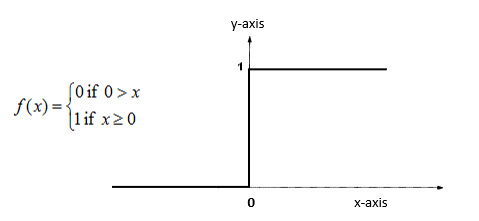
\includegraphics[height=3cm]{Pictures/activation-fns/step-function.jpg}
    \caption{Activation Function: Step Function}
\end{figure}

\[
    y={\begin{dcases}1&{\text{if }}u\geq \theta \\0&{\text{if }}u<\theta \end{dcases}}
\]

\begin{enumerate}
    \item The output y of this transfer function is binary, depending on whether the input meets a specified threshold, $\theta$. 
    \item The "signal" is sent, i.e. the output is set to one, if the activation meets the threshold.
    \item It performs a division of the space of inputs by a hyperplane. 
    \item It is specially useful in the last layer of a network intended to perform binary classification of the inputs. 
    \item It can be approximated from other sigmoidal functions by assigning large values to the weights.
\end{enumerate}

\section{Infinite Step Function ( $1(z)$ )}

\[
    1(z) = {\begin{dcases}
        0 & \text{ if } z \leq 0 \\
        \infty & \text{ otherwise }
    \end{dcases}}
\]

This gives infinite penalty if the constraint is not satisfied.


\section{Sigmoid function \cite{wiki-activation-fn,wiki-Sigmoid_function}} \label{Sigmoid function: broad section}

\begin{enumerate}
    \item A sigmoid function is any mathematical function whose graph has a characteristic S-shaped or sigmoid curve.
    \item A sigmoid function is a bounded, differentiable, real function that is defined for all real input values and has a non-negative derivative at each point and exactly one inflection point.
    \item A sigmoid function is monotonic, and has a first derivative which is bell shaped
    \item The integral of any continuous, non-negative, bell-shaped function (with one local maximum and no local minimum, unless degenerate) will be \textbf{sigmoidal}.
    \item A sigmoid function is constrained by a pair of \textbf{horizontal asymptotes} as $x\rightarrow \pm \infty$
    \item A sigmoid function is \textbf{convex} for values less than a particular point, and it is \textbf{concave} for values greater than that point: in many of the examples here, that point is 0.
\end{enumerate}

\subsection{Logistic function ( $\sigma(x)$ ) \cite{wiki-Logistic_function,wiki-Sigmoid_function}}\label{Logistic function}

\begin{figure}[H]
    \centering
    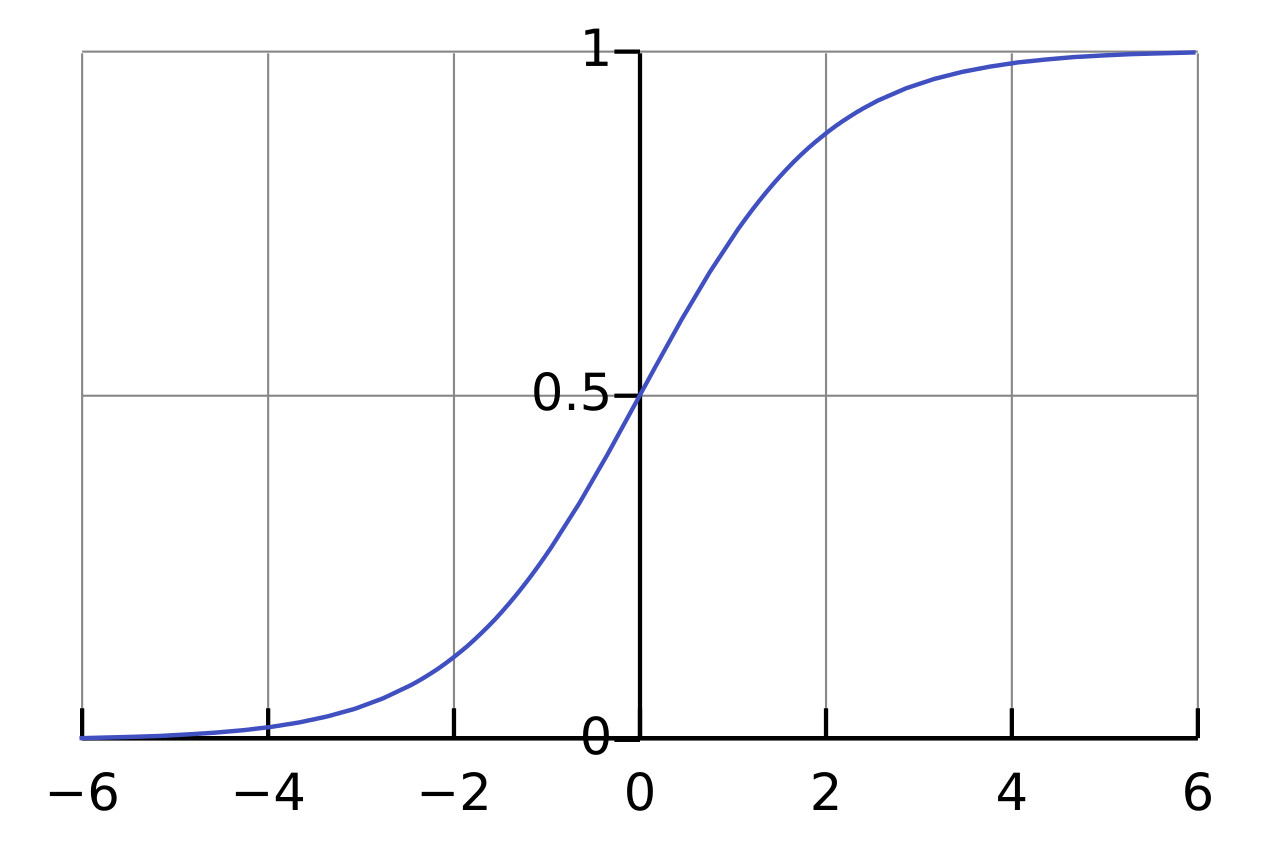
\includegraphics[height=3cm]{Pictures/activation-fns/sigmoid-fn.jpg}
    \caption{Activation Function: Sigmoid Function}
\end{figure}

\subsubsection{General Equation \cite{wiki-Logistic_function,wiki-Sigmoid_function}}
\[
    f(x) = {\dfrac{L}{1 + e^{-k(x - x_{0})}}}
\]


\vspace{0.2cm}

\begin{enumerate}
    \item $L$ is the carrying capacity, the supremum of the values of the function
    \item $k$ is the logistic growth rate, the steepness of the curve
    \item $x_{0}$ is the $x$ value of the function's midpoint
\end{enumerate}


\subsubsection{Standard logistic function (sigmoid/ expit) \cite{wiki-Logistic_function,wiki-Sigmoid_function,dnn-1}}  \label{sigmoid}\label{expit}\label{Standard logistic function}
\[
    \sigma(x) 
    = {\dfrac{1}{1+e^{-x}}} 
    = {\dfrac{e^{x}}{1+e^{x}}} 
    = 1- \sigma(-x)
    \hfill
    (L=1 , k=1 \& x_{0}=0)
\]

\[
    \dfrac{d}{dx} \sigma(x) 
    = \dfrac{\exp(-x)}{(1 + \exp(-x))^2} 
    = \sigma(x)\left(1-\sigma(x)\right)
    = \sigma(x)\sigma(-x)
    \hfill\text{\cite{dnn-deep-learning-ian}}
\]

\[
    \log(\sigma(x))
    = -\zeta(-x)
    \hfill \text{\fullref{SmoothReLU/ Softplus}}
    \hfill \text{\cite{dnn-deep-learning-ian}}
\]
\[
    \forall x \in (0,1), \ 
    \sigma^{-1}(x)
    = \log\dParenBrac{\dfrac{x}{1-x}}
    \hfill\text{\cite{dnn-deep-learning-ian}}
\]

\begin{enumerate}
    \item when the input is close to $0$, the sigmoid function approaches a linear transformation

    \item when the input is $0$, the derivative of the sigmoid function reaches a \textbf{maximum} of $0.25$. As the input diverges from $0$ in either direction, the derivative approaches $0$.

    \item sigmoid’s gradient vanishes both when its inputs are large and when they are small. 
    
    \item when backpropagating through many layers where the inputs to many of the sigmoids are close to zero, the gradients of the overall product may vanish.

\end{enumerate}


\section{Softmax function/ softargmax ( $\sigma (\mathbf {z})$ ) \cite{wiki-softmax-function,dnn-1}} \label{Softmax function}
\begin{enumerate}
    \item The softmax function, also known as softargmax or normalized exponential function, converts a vector of $K$ real numbers into a probability distribution of $K$ possible outcomes. 
    
    \item It is a generalization of the logistic function to multiple dimensions, and used in multinomial logistic regression. 
    
    \item The softmax function is often used as the last activation function of a neural network to normalize the output of a network to a probability distribution over predicted output classes.

    \item $
        {\displaystyle \sigma (\mathbf {z} )_{i}={\displaystyle\dfrac {\exp({z_{i}})}{\dsum _{j=1}^{K} \exp({z_{j}})}}}
    $\\
    Where:
    \[
        {\displaystyle \sigma \colon \mathbb {R} ^{K}\to (0,1)^{K}}
        \hfill
        {\displaystyle K\geq 1}
    \]
    \[
        {\displaystyle \mathbf {z} =(z_{1},\dotsc ,z_{K})\in \mathbb {R} ^{K}}
    \]

    \item \textbf{numerical overflow}: If some of the $z_j$ are very large, i.e., very positive, then $\exp(z_j)$ might be larger than the largest number we can have for certain data types. This is called overflow.
    
    \item \textbf{numerical underflow}: if every argument is a very large negative number, we will get underflow.
    
    \item A way round this problem is to subtract $\bar{o} \stackrel{\textrm{def}}{=} \max_k o_k$ from all entries:
    \[
        \hfill
        \hat y_j 
        = \dfrac{\exp (o_j)}{\dsum_k \exp (o_k)} 
        = \dfrac{\exp(o_j - \bar{o}) \exp (\bar{o})}{\dsum_k \exp (o_k - \bar{o}) \exp (\bar{o})} 
        = \dfrac{\exp(o_j - \bar{o})}{\dsum_k \exp (o_k - \bar{o})}
        \hfill
        (o_j - \bar{o} \leq 0 \quad \forall j)
    \]
    denominator: $\in [1, q]$\\
    numerator: $\leq 1$ \\
    \[
        \hfill
        \log (\hat{y}_j )
        = \log \dParenBrac{\dfrac{\exp(o_j - \bar{o})}{\dsum_k \exp (o_k - \bar{o})} }
        = o_j - \bar{o} - \log \dParenBrac{\dsum_k \exp (o_k - \bar{o})}
        \hfill
    \]
    
\end{enumerate}


\section{Rectifier/ Rectified Linear Unit ( $\operatorname{ReLU}(x)$ ) \cite{wiki-Rectifier,dnn-1}}\label{ReLU}
In the context of artificial neural networks, the rectifier or ReLU (rectified linear unit) activation function is an activation function defined as the positive part of its argument:
\[
    \operatorname{ReLU}(x)=x^{+}=\max(0,x)={\dfrac {x+\dabs{x}}{2}}
    ={\begin{dcases}x&{\text{if }}x>0\\
    0&{\text{otherwise}}\end{dcases}}
\]
\[
    \dfrac{d\operatorname{ReLU}(z)}{dz}={\begin{dcases}1&{\text{if }}z>0,\\0&{\text{otherwise}}\end{dcases}}
\]

\section{Leaky ReLU \cite{wiki-Rectifier}}\label{Leaky ReLU}
Leaky ReLUs allow a small, positive gradient when the unit is not active, helping to mitigate the vanishing gradient problem
\[
    f(x)
    = \max(x,0) + \alpha\cdot\min(x,0)
    ={\begin{dcases}x&{\text{if }}x>0,\\\alpha\cdot x&{\text{otherwise}}\end{dcases}} 
\]

$\alpha$ is a constant

\section{Parametric ReLU ($\operatorname{pReLU}(x)$) \cite{wiki-Rectifier,dnn-1}} \label{Parametric ReLU (PReLU)}
Parametric ReLUs (PReLUs) take this idea further by making the coefficient of leakage into a parameter that is learned along with the other neural-network parameters
\[
    \operatorname{pReLU}(x)
    = \max(x,0) + a\cdot\min(x,0)
    ={\begin{dcases}x&{\text{if }}x>0,\\a\cdot x&{\text{otherwise}}\end{dcases}}
\]

$a$ is a learnable parameter

\section{Gaussian-error linear unit (GELU)}\label{Gaussian-error linear unit (GELU)}
GELU is a smooth approximation to the rectifier
\[
    f(x)=x\cdot \Phi (x)
\]
\[
    f'(x)=x\cdot \Phi '(x)+\Phi (x)
\]

$\Phi (x)$ is Standard Normal Function


\section{Sigmoid linear unit/ Swish function (SiLU)}\label{Sigmoid linear unit/ Swish function (SiLU)}
The SiLU (sigmoid linear unit) or swish function is another smooth approximation, first coined in the GELU paper.
\[
    f(x)=x\cdot \operatorname {sigmoid} (x)
\]
\[
    f'(x)=x\cdot \operatorname {sigmoid} '(x)+\operatorname {sigmoid} (x)
\]

SEE \fullref{sigmoid}

\section{SmoothReLU/ Softplus ($\zeta(x)$) \cite{wiki-Rectifier}}\label{SmoothReLU/ Softplus}
A smooth approximation to the rectifier is the analytic function.
\[ 
    \zeta(x)=\ln(1+e^{x}) 
    \hfill\text{\cite{dnn-deep-learning-ian}}
\]
\[
    \zeta'(x)
    ={\dfrac {e^{x}}{1+e^{x}}}={\displaystyle \dfrac {1}{1+e^{-x}}} 
    \hfill\text{\cite{dnn-deep-learning-ian}}
\]
\[ 
    \zeta(x)
    =\ln \left(1+e^{x}\right)
    \approx {\begin{dcases}\ln 2,&x=0,\\[6pt]{\displaystyle \dfrac {x}{1-e^{-x/\ln 2}}},&x\neq 0\end{dcases}} 
\]
\[
    \zeta(x)
    = \dint_{-\infty}^{x} \sigma(y)dy
    \hfill\text{\cite{dnn-deep-learning-ian}}
\]
\[
    \zeta(x) - \zeta(-x) = x
    \hfill\text{\cite{dnn-deep-learning-ian}}
\]

smoothed or “softened” version of $x^+ = \max(0,x)$

\[
    \dfrac{d}{dx}\dParenBrac{\zeta(x)}
    = \sigma(x)
    \hfill\text{\cite{dnn-deep-learning-ian}}
\]
\[
    \forall x > 0,\ 
    \zeta^{-1}(x) = \log(e^x-1)
    \hfill\text{\cite{dnn-deep-learning-ian}}
\]

\section{Exponential linear units (ELU) \cite{wiki-Rectifier}}\label{Exponential linear units (ELU)}
Exponential linear units try to make the mean activations closer to zero, which speeds up learning. It has been shown that ELUs can obtain higher classification accuracy than ReLUs.
\[
    {\displaystyle f(x)={\begin{dcases}x&{\text{if }}x>0,\\a\left(e^{x}-1\right)&{\text{otherwise}}.\end{dcases}}\qquad \qquad f'(x)={\begin{dcases}1&{\text{if }}x>0,\\a\cdot e^{x}&{\text{otherwise}}.\end{dcases}}}
\]

In these formulas, \(\displaystyle a\) is a hyper-parameter to be tuned with the constraint \(\displaystyle a\geq 0\).

\section{Mish \cite{wiki-Rectifier}}\label{Mish}
The mish function can also be used as a smooth approximation of the rectifier
\[
    \displaystyle f(x)=x\tanh {\big (}\rcmdXsoftplus (x){\big )}
\]
where \({\displaystyle \tanh(x)}\) is the hyperbolic tangent, and \({\displaystyle \rcmdXsoftplus(x)}\) is the softplus function.\par
Mish is non-monotonic and self-gated. It was inspired by Swish, itself a variant of ReLU.

\section{Squareplus \cite{wiki-Rectifier}}\label{Squareplus}
\[
    {\displaystyle \operatorname {squareplus} _{b}(x)={\dfrac {x+{\sqrt {x^{2}+b}}}{2}}}
\]

where \({\displaystyle b\geq 0}\) is a hyperparameter that determines the "size" of the curved \({\displaystyle x=0}\).

\begin{enumerate}
    \item $b=0$ yields ReLU
    \item It is monotonic, strictly positive, approaches 0 as \({\displaystyle x\to -\infty }\), approaches the identity as \({\displaystyle x\to +\infty }\), and is \({\displaystyle C^{\infty }}\) smooth.
    \item squareplus can be computed using only algebraic functions, making it well-suited for settings where computational resources or instruction sets are limited.
    \item squareplus requires no special consideration to ensure numerical stability when \({\displaystyle x}\) is large.
\end{enumerate}



\section{Convolution ( $(f * g)(\mathbf{x})$ ) \cite{dnn-1}} \label{function: Convolution}

\begin{enumerate}
    \item In mathematics, the convolution between two functions, say $f, g: \mathbb{R}^d \to \mathbb{R}$ is defined as:
    \[
        \hfill
        (f * g)(\mathbf{x}) = 
        \begin{dcases}
            \dint f(\mathbf{z}) g(\mathbf{x}-\mathbf{z}) d\mathbf{z} & \text{ (continuous)} \\[1ex]
            \dsum_\mathbf{z} f(\mathbf{z}) g(\mathbf{x}-\mathbf{z}) & \text{ (discrete)} \\
        \end{dcases}
        \hfill
    \]
    we measure the overlap between $f$ and $g$ when one function is “\textbf{flipped}” and \textbf{shifted} by $\mathbf{x}$

    \item For two-dimensional tensors, we have a corresponding sum with indices $(a, b)$ for $f$ and $(i - a, j - b)$ for $g$:
    \[
        \hfill
        (f * g)(i, j) = \dsum_a\dsum_b f(a, b) g(i-a, j-b)
        \hfill
    \]
\end{enumerate}



